%\section{Class Diagram}
\section{Component architecture}

The architecture of the administrations part of the Giraf system is designed as a client-server architecture. Which means that the user uses the client to communicate with the server, at which the database lies. Within the client and the server lie three components. These components are called; view, controller and database. These three components communicate with each other in the way that the the view communicates with the database through the controller. Which means that the controller is the link between the two other components. Even though the architecture of the system is client-server, it is designed such that the client does not contain any components, and therefore the server contain all the three components, the reason is that the system is 100\% internet based and is utilized by means of an internet browser. The componentarchitecture can be seen in Figure \vref{fig:architecture}

\begin{figure}[!ht]
\centering
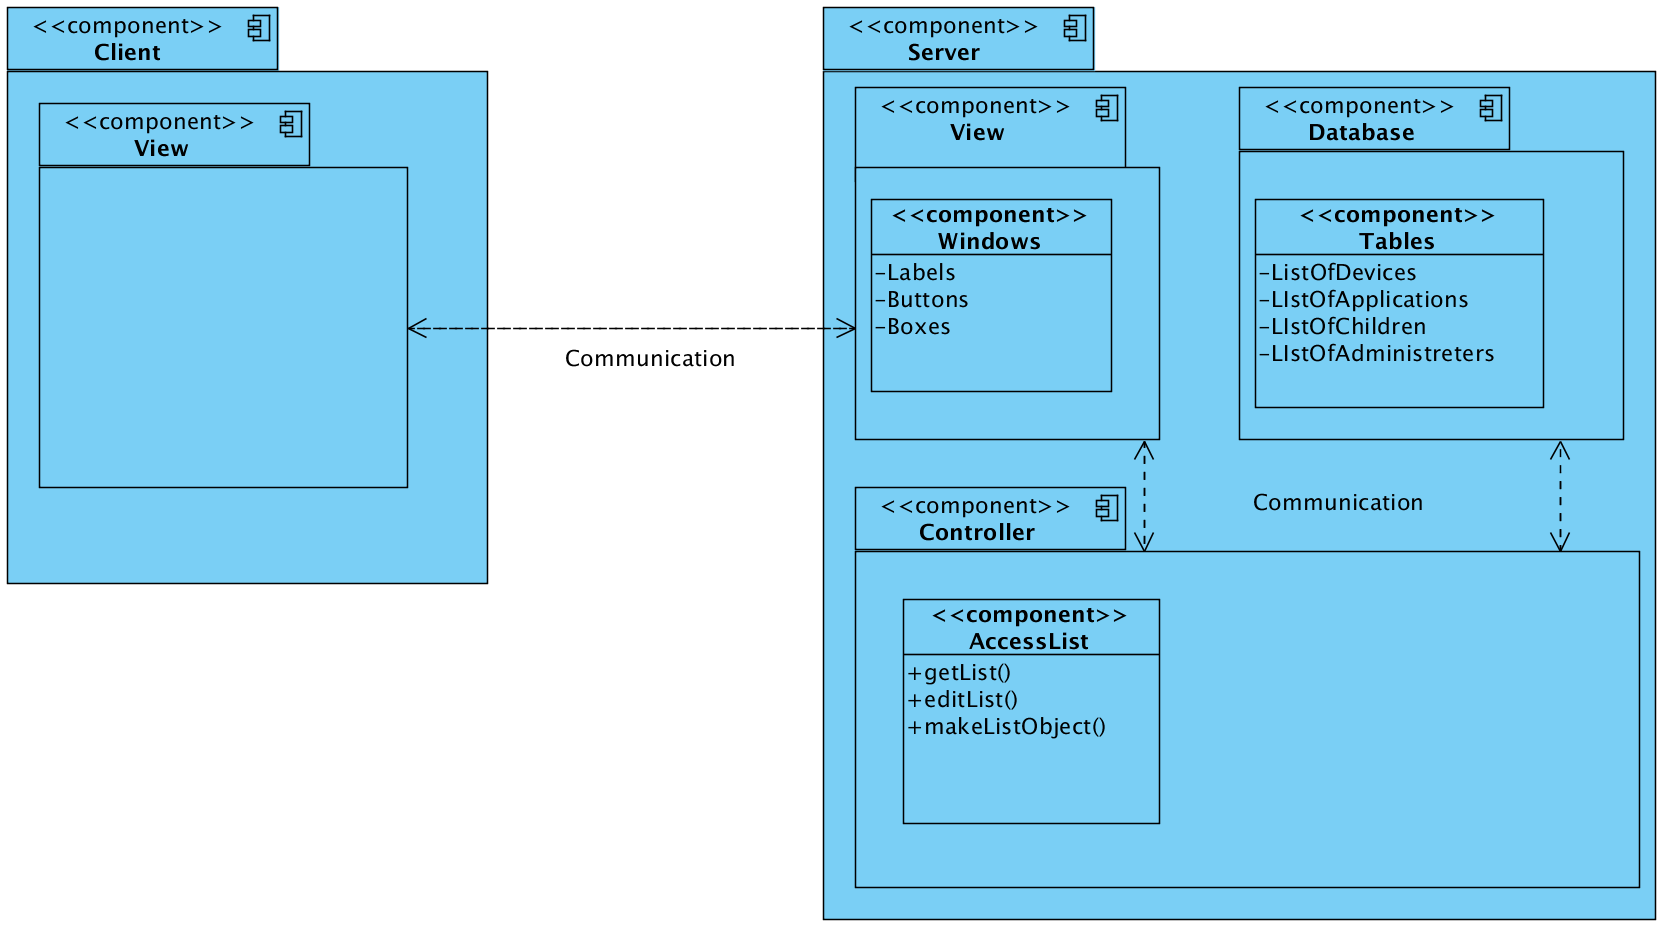
\includegraphics[width=300px]{img/ComponentArketektur.png}
\caption{The figure shows the component architecture of the administrations system}
\label{fig:architecture}
\end{figure}

The three components contain other components, which contain some attributes. These attributes define what function the overall component has, for example contains the view component a windows component, which contains some attributes called 'labels', 'buttons' and 'boxes'.The attributes show that the windows component can indicate labels, buttons and boxes.
The controller contains a component with some attributes which indicates that the accesList can, get a list from the database, edit a list from the database and make an object of a list.
The database component contains a component called lists, this component has an attribute called lists, this attribute indicates that the database contains lists. Among these lists is a list of devices, a list of children, a list of applications and a list of administrators.